\documentclass[crop,tikz]{standalone}
\usetikzlibrary{backgrounds}
\colorlet{blue}{cyan}
\tikzset{
  inverted/.style = {
    every path/.style = {draw=white,text=white},
    background rectangle/.style={fill},
    show background rectangle
  }
}

\usepackage{amsmath}
\usetikzlibrary{calc}
\tikzset{>=latex}
\newcommand{\F}{\vec{F}}

\newcommand{\bigship}[3]{%
  \begin{scope}[shift={#1}, scale={#2/10}, rotate=#3, xscale=-1]
    \draw[fill=white, rounded corners=1] (0,0) -- ++(1,-1) -- ++(9,0) -- ++(0,1) -- cycle;%
    \draw[fill=white, rounded corners=1] (7,0.1) rectangle ++(2,0.7);%
  \end{scope}
}

\newcommand{\smallship}[3]{%
  \begin{scope}[shift={#1}, scale={#2/2}, rotate=#3, xscale=-1]
    \draw[fill=white, rounded corners=1] (0,0) -- ++(0.7,-1) -- ++(2,0) -- ++(0,1) -- cycle;%
    \draw[fill=white, rounded corners=1] (1.6,0) rectangle ++(1,0.4);%
  \end{scope}
}

\begin{document}
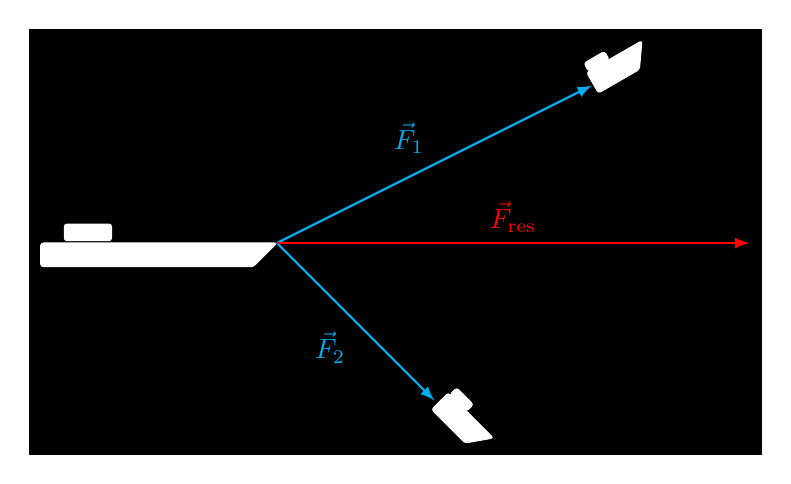
\begin{tikzpicture}[inverted,inverted]
  \bigship{(0,0)}{3}{0}
  \smallship{(-42:3.7)}{0.6}{-45}
  \smallship{(29:5.3)}{0.6}{30}
  % arrows
  \draw[->, blue, thick] (0,0) -- node[above left] {$\F_1$} (4,2) coordinate (F1);
  \draw[->, blue, thick] (0,0) -- node[below left] {$\F_2$} (2,-2) coordinate (F2);
  \draw[->, red , thick] (0,0) -- node[above] {$\F_\text{res}$} ($(F1)+(F2)$);
\end{tikzpicture}
\end{document}
